\subsection{The structure of the feature space}
\label{ch:structure}

The sixty-one hand-made features of \cref{sec:prep:features} (listed in \cref{app:features})
were built to feed the stateless control of \cref{ch:stateless}, and the experiments use
them only through the accuracy of what is trained on them.  They are defined in
\cref{sec:prep:features} and taken as given here, because what is asked of them does not need a trained
forecaster.  This section looks at the features themselves,
with the tools of classical data mining, and asks four questions that do not need a
trained forecaster: how many independent quantities the features really contain; whether
the label is organised geometrically in the feature space, or whether the space is
organised by something else; how much of the separability is linear, how much is local and
how much needs interactions; and whether the markets form natural families that cut across
the categories of \cref{sec:expl:templates}.  The answers set expectations for every model
family and explain, before any training, several of the results of
\cref{ch:stateless,ch:stateful,ch:horizons}.

Everything in this section uses the samples of the validation day, 13 March, with the
training rows of 7--12 March wherever a method is fitted, and never the test set
(\cref{sec:data:protocol}).  The methods are the standard implementations of scikit-learn
\cite{pedregosa2011sklearn} and umap-learn \cite{mcinnes2018umap}; the script is
\path{scripts/data_audit/datamining.py} (\cref{app:reproduction}).  The horizon of 15
minutes is used as the reference throughout, because its classes are the least unbalanced
of the short horizons (\cref{tab:expl:classes}); the same study was run at every horizon
and the differences are reported where they matter.

\subsubsection{Preprocessing}
\label{sec:structure:prep}

Distance-based methods need the features on a common scale and without the heavy tails
that order-book quantities have.  Every feature is imputed with its training median and
then mapped by rank through the inverse normal distribution (a rank-gauss transform, fitted
on one million training rows): a monotone map, so that trees and rules are unaffected,
which gives every feature the same marginal distribution.  Fifty-nine features enter the
analysis: the hand-made features of \cref{sec:prep:features} without the category of the
market, one of eight classes derived from the tags that Polymarket attaches to each market
(\cref{sec:data:collection}), which is kept as a label to colour by and never as an
input, and without the time since the last book event, which is constant on the training
rows.

\subsubsection{How many quantities the features contain}
\label{sec:structure:dim}

\begin{figure}[t]
\centering
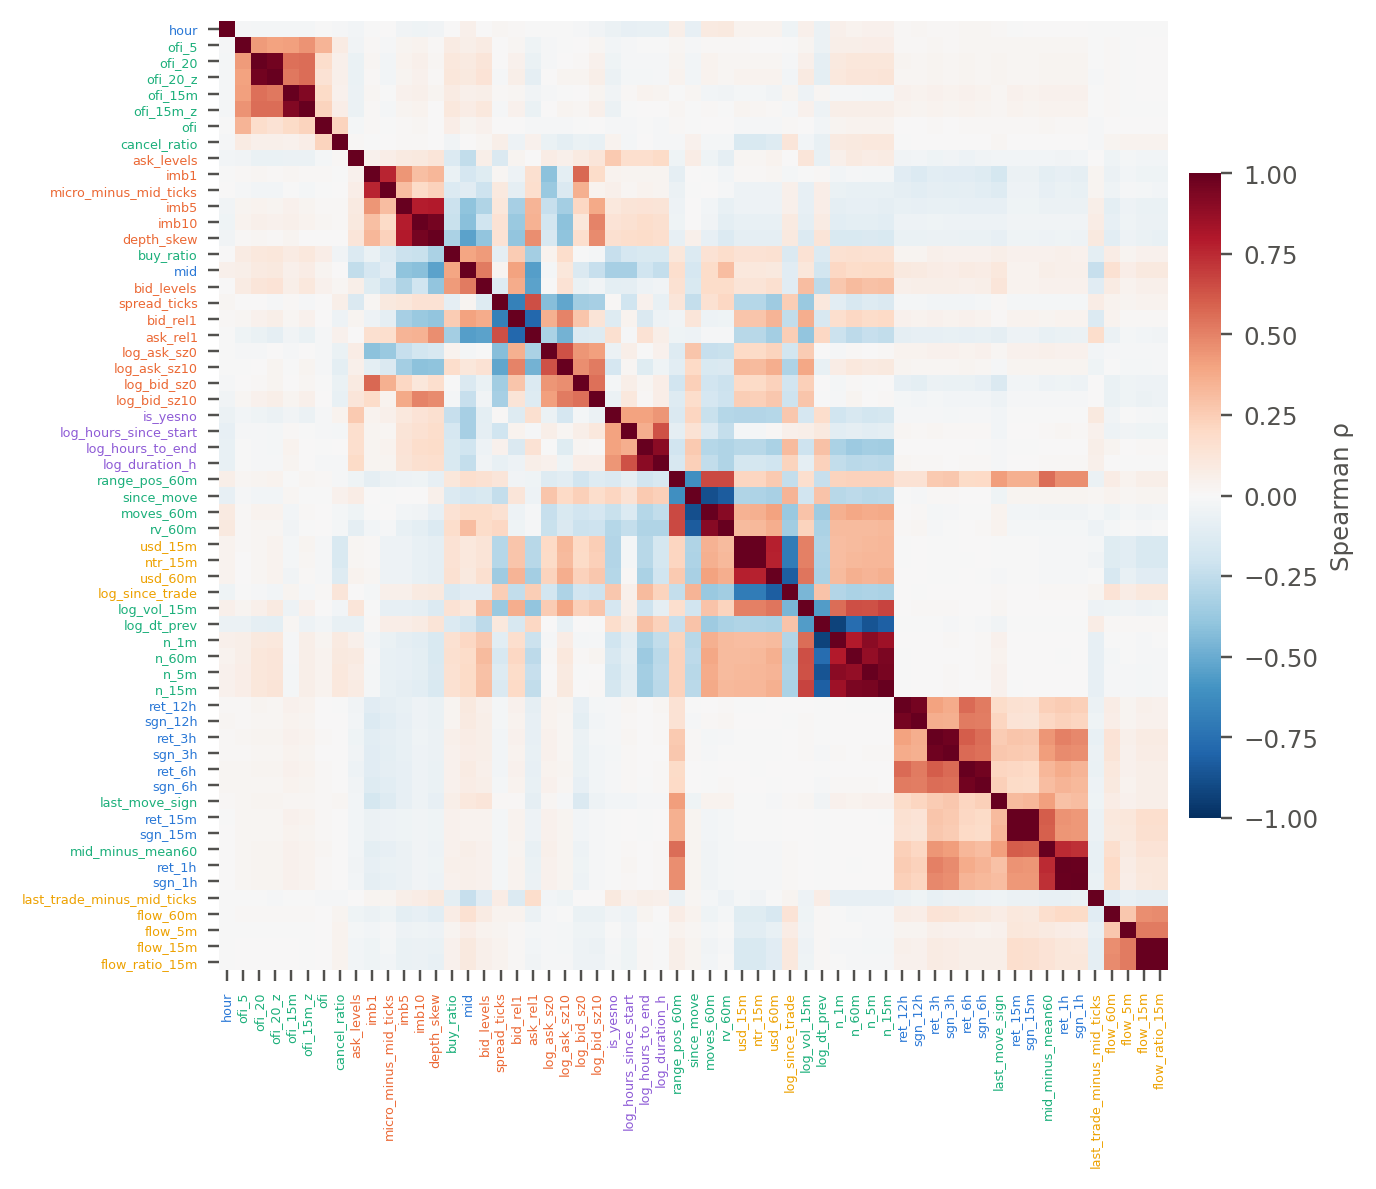
\includegraphics[width=\textwidth]{figures/dm/dm_corr_15m.png}
\caption{Spearman correlation of the fifty-nine features on 200{,}000 validation samples
at 15 min, ordered by average-linkage clustering of $1 - |\rho|$.  Tick labels are coloured
by group: blue G1 price, orange G2 book, aqua G3 flow and clock, yellow G4 trades, violet G5
static.  The blocks are the returns with their signs, the event counts, the order-flow
imbalances with their standardised copies, the on-chain trade quantities, and the
sixty-minute activity triple.}
\label{fig:structure:corr}
\end{figure}

\paragraph{Principal components.}  On 200{,}000 validation samples at 15 min, four
principal components hold half of the variance, ten hold 80\% and twenty-three hold 95\%;
the participation ratio of the spectrum, the number of equally loaded components that
would give the same spread, is $9.7$.  The first component (23\% of the variance) is the
direction of the recent history: it loads on the sign of the last move and on the signs of
the 3, 6 and 12-hour changes.  The second (14\%) is activity: the sixty-minute realised
volatility, the number of moves, the dollars traded and the position in the sixty-minute
range.  The third (10\%) opposes the sign of the last move to the long signs, which is a
reversal axis, and the fourth (7\%) opposes activity to trades.  By group, the price and
the flow-and-clock features take almost all of the first six components; the book-shape
features (G2) take between 0.3\% and 9\% of each.  The book shape is a low-variance
direction of the space, because its quantities are bounded ratios, and a method that looks
for variance will not find it; whether it carries information is a different question,
answered below by the mutual information.

\paragraph{Correlation blocks.}  \Cref{fig:structure:corr} shows the Spearman correlation
matrix.  The participation ratio of its spectrum, an effective number of independent
features, is $16.8$.  At $|\rho| \ge 0.7$ the features fall into fifteen blocks of two to
five: each return with its sign; the event counts over 1, 5, 15 and 60 minutes with the
time since the previous row; the two order-flow imbalances with their standardised copies;
the dollars and the number of on-chain trades with the time since the last trade; the
sixty-minute number of moves, realised volatility and time since the last move; the
imbalances at five and ten levels with the depth skew; the hours to the end with the
duration of the market.  At $|\rho| \ge 0.9$ fourteen pairs remain.  The fifty-nine columns
are, in short, about seventeen quantities, and a model that reads all of them is reading
each of these quantities three or four times.

\paragraph{Random projection and multidimensional scaling.}  A Gaussian random
projection to twenty dimensions preserves the pairwise distances of 3{,}000 samples within
a ratio of $0.75$ to $1.36$ (5th and 95th percentile; standard deviation $0.18$), and to
forty dimensions within $0.82$ to $1.18$; a nearest-neighbour classifier on the
twenty-dimensional projection loses $0.65$ points of balanced accuracy against the same
classifier on the full space (\cref{sec:structure:sep}).  The intrinsic dimension is
therefore well below fifty-nine but well above two: a metric multidimensional scaling of
2{,}000 samples to the plane has a Kruskal stress of $0.31$, against $0.48$ for the first
two principal components on the same rows, and both are far from a faithful planar map.

\subsubsection{Maps of the samples}
\label{sec:structure:maps}

\begin{figure}[p]
\centering
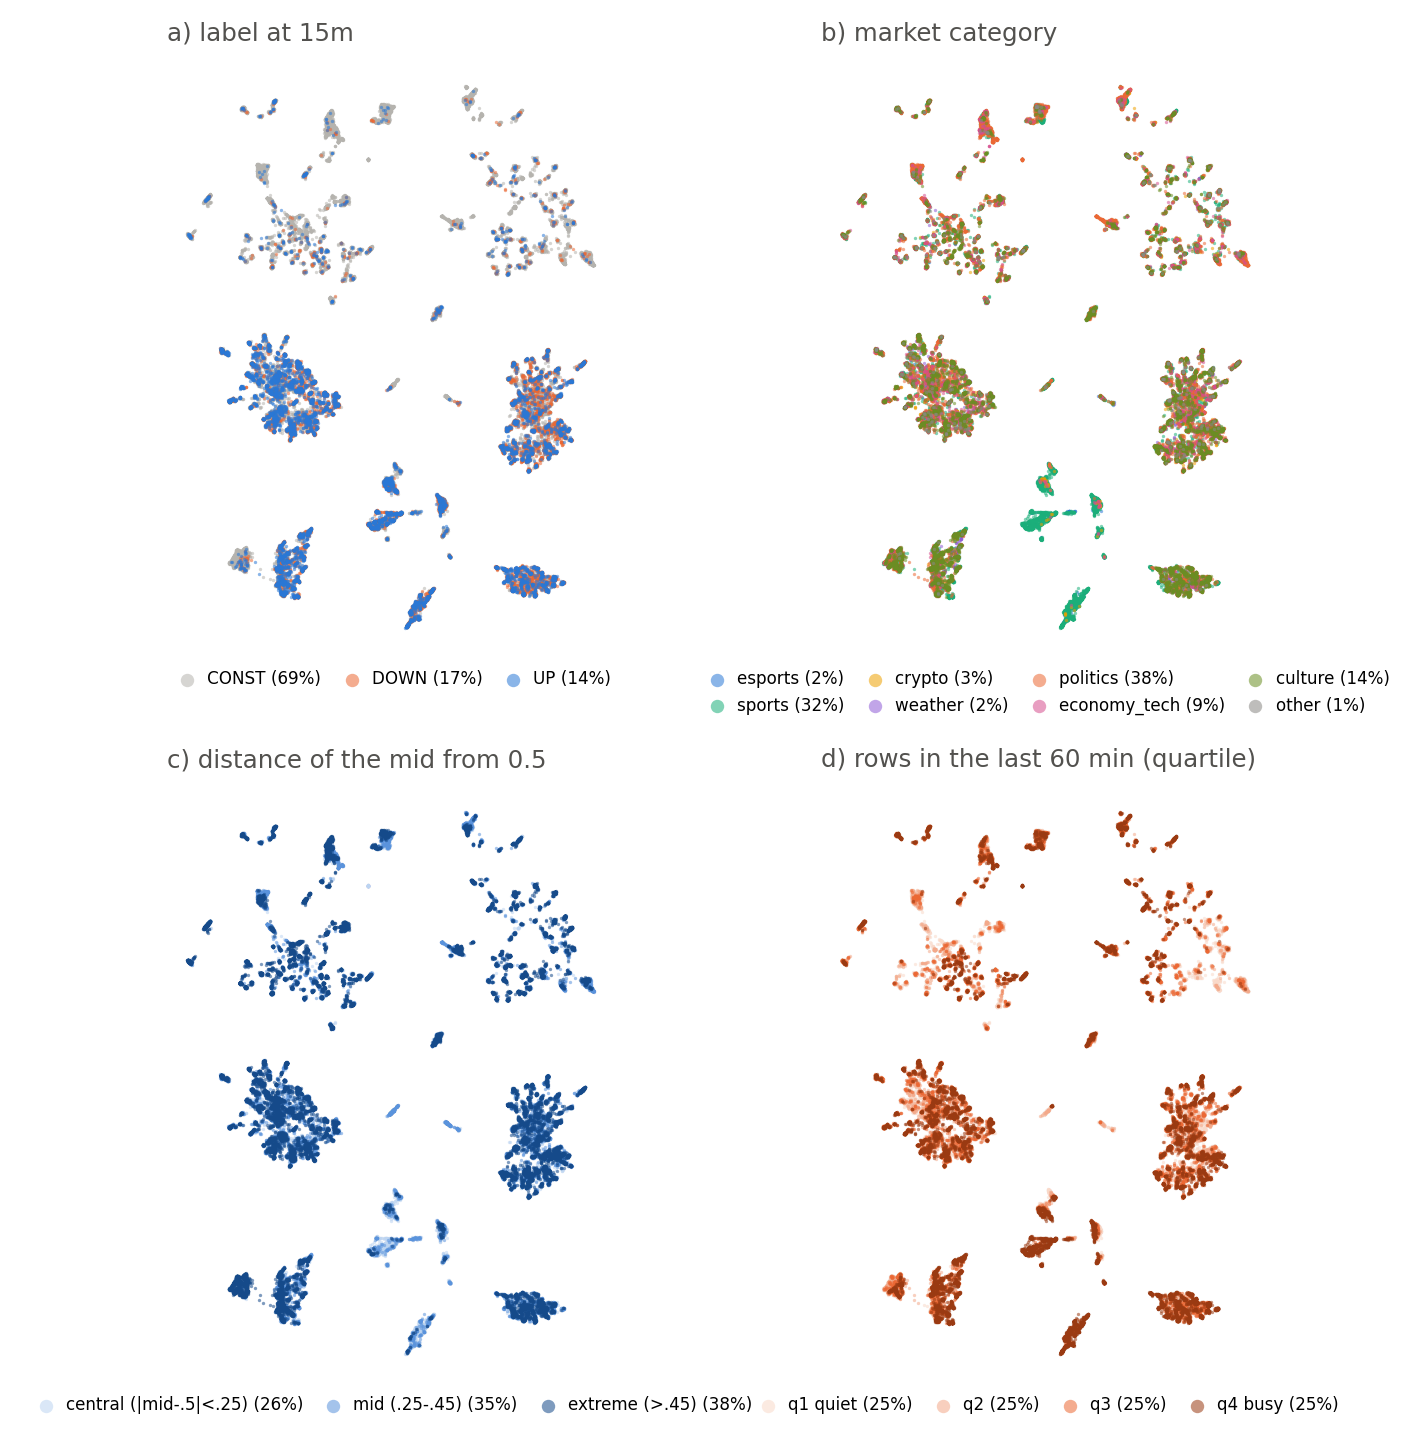
\includegraphics[width=\textwidth]{figures/dm/dm_umap_15m.png}
\caption{UMAP of 50{,}000 validation samples at 15 min (fifty-nine rank-gauss features,
thirty neighbours), the same points coloured four ways: (a) the label at 15 min, (b) the
category of the market, (c) the distance of the mid from one half, (d) the quartile of
the number of book rows in the last sixty minutes.  The islands are coherent in activity
and, largely, in category; the label is spread inside each island.}
\label{fig:structure:umap}
\end{figure}

\Cref{fig:structure:umap} is a UMAP of 50{,}000 samples and \cref{tab:structure:purity}
measures what the map, and the original space, are organised by: for each sample, the
share of its fifteen nearest neighbours that carry the same label, divided by the share
expected by chance.  The lift of the prediction label is $1.24$ in the map and $1.26$ in
the fifty-nine-dimensional space: the neighbours of a sample that is about to move are
only a quarter more likely than chance to move as well.  The lift of the activity quartile
is $1.7$ to $1.9$, that of the price-level bucket $1.4$ to $1.6$, that of the category
$1.5$ to $1.7$, and that of the market identity is $100$ to $200$: one neighbour in twenty
comes from the same market, out of eleven thousand.  The feature space is organised by the
market and by its activity, not by what the price is about to do; the label is a weak
modulation on top of a geometry made of market regimes.  UMAP and t-SNE keep between 85\%
and 95\% of the lifts of the original space, so the maps are faithful to this extent, and
the two methods agree with each other on every count.

\begin{table}[t]
\centering
\caption{Neighbourhood purity in the maps and in the original space at 15 min: share of
the fifteen nearest neighbours with the same label, the share expected by chance
($\sum_c p_c^2$) and their ratio.  UMAP on 50{,}000 samples, t-SNE on 20{,}000.}
\label{tab:structure:purity}
\small
\begin{tabular}{lccc ccc}
\toprule
& \multicolumn{3}{c}{UMAP} & \multicolumn{3}{c}{original space} \\
\cmidrule(lr){2-4}\cmidrule(lr){5-7}
Label & same & chance & lift & same & chance & lift \\
\midrule
prediction label (3 classes) & 0.649 & 0.524 & 1.24 & 0.662 & 0.524 & 1.26 \\
market category (8)          & 0.404 & 0.273 & 1.48 & 0.462 & 0.273 & 1.69 \\
price-level bucket (3)       & 0.488 & 0.341 & 1.43 & 0.556 & 0.341 & 1.63 \\
activity quartile (4)        & 0.423 & 0.250 & 1.69 & 0.487 & 0.250 & 1.95 \\
market identity (11{,}294)   & 0.026 & 0.0003 & 104 & 0.052 & 0.0003 & 202 \\
\bottomrule
\end{tabular}
\end{table}

The picture explains two results of the experiments.  The same-market lift is why the
per-market state of \cref{ch:stateful} has something to learn, and why deduplication
changes every number: consecutive samples of a market are neighbours in the feature space
and carry nearly the same information.  The weak label lift is why no family reaches
balanced accuracies far above $0.6$ at this horizon: in the space of what is observable
at the sample time, samples that will move and samples that will not are mixed at the
scale of fifteen neighbours.

\subsubsection{Linear, local and interaction separability}
\label{sec:structure:sep}

\begin{table}[t]
\centering
\caption{Separability of the three classes at 15 min on the validation day, balanced
accuracy on all and on deduplicated samples.  Linear models and trees are fitted on one
million training rows; kNN on the same rows and evaluated on 300{,}000 validation samples,
with the vote of the neighbours weighted by the inverse class frequency.  LightGBM is the
G5 control of \cref{ch:stateless}, uncalibrated.}
\label{tab:structure:sep15}
\small
\begin{tabular}{lcc}
\toprule
Model & all & dedup \\
\midrule
Mean Reversion-$H$                      & 0.537 & 0.525 \\
LDA, uniform priors                     & 0.561 & 0.495 \\
Logistic regression, balanced weights   & 0.568 & 0.505 \\
Decision tree, depth 3, balanced        & 0.548 & 0.549 \\
Decision tree, depth 6, balanced        & 0.571 & 0.562 \\
kNN, $k = 5$                            & 0.532 & 0.517 \\
kNN, $k = 50$                           & 0.570 & 0.551 \\
kNN, $k = 200$                          & 0.574 & 0.553 \\
kNN, $k = 1000$                         & 0.572 & 0.551 \\
kNN, $k = 50$, 20-D random projection   & 0.564 & 0.547 \\
LightGBM G5 (control)                   & 0.616 & 0.600 \\
\bottomrule
\end{tabular}
\end{table}

\Cref{tab:structure:sep15} places the classical learners between Mean Reversion and
the control.  Three things stand out.

\paragraph{The linear signal is ``whether'', and it lives in the busy markets.}  Linear
discriminant analysis and a balanced logistic regression gain $2.3$ and $3.0$ points over
Mean Reversion on all samples and \emph{lose} $3$ and $2$ points on the deduplicated
samples.  The leading discriminant direction is made of the number of trades and of book
events in the last minutes, the time since the last move and the number of moves in the
hour, with the sign structure of an activity axis: it separates \textsc{const} from the
two moving classes, and it does so on the stream of consecutive samples of busy markets,
which deduplication removes.  \Cref{fig:structure:lda} shows it: the \textsc{const}
samples form a cloud on the right of LD1, the moving samples a wider cloud on the left,
and \textsc{down} and \textsc{up} overlap almost completely.  A linear function of the
features cannot tell the direction; it can tell, imperfectly, the activity.

\begin{figure}[t]
\centering
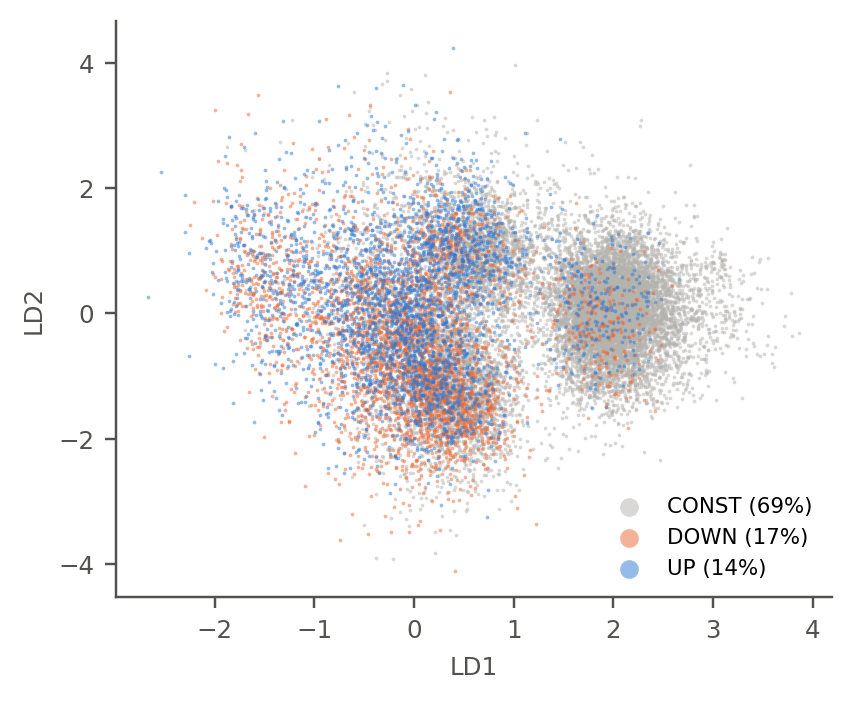
\includegraphics[width=0.62\textwidth]{figures/dm/dm_lda_15m.png}
\caption{The two discriminant directions of LDA at 15 min on 20{,}000 validation samples.
LD1 separates \textsc{const} (right) from the moving classes (left); the two directions
overlap.}
\label{fig:structure:lda}
\end{figure}

\paragraph{Thresholds and a few interactions do most of the work.}  A depth-three tree,
twelve numbers in all, reaches $0.548$ on all samples and $0.549$ deduplicated, above every
linear model on the deduplicated samples; a depth-six tree reaches $0.571$ and $0.562$.
The depth-three tree is worth reading in full, because it is the simplest statement of what
the short-horizon problem is:

\begin{quote}\small\ttfamily
\begin{tabular}{@{}l@{}}
since\_move $\le$ 1048 s (the price moved in the last 17 minutes)\\
\quad moves\_60m $\le$ 8.5: last\_move\_sign $\le 0$ $\to$ \textsc{up}, else \textsc{down}\\
\quad moves\_60m $>$ 8.5: since\_move $\le$ 121 s $\to$ \textsc{up}, else \textsc{down}\\
since\_move $>$ 1048 s $\to$ \textsc{const} on every branch
\end{tabular}
\end{quote}

The first split is the activity clock of \cref{sec:expl:activity}: if the price has not
moved in the last seventeen minutes, predict that it will not move.  Below it, in the
quieter markets, the direction is the reversal of the last move, which is Mean Reversion
on the last tick; in the busier markets the tree uses the recency of the last move
instead, a split that balanced weighting rewards and that the full learners do not keep.
The gap from this tree to the control, $6.8$ points on all samples and $5.1$
deduplicated, is what six hundred boosted trees of sixty-three leaves add: finer
thresholds on the same quantities and interactions between the activity, the price level
and the book.

\paragraph{Local information is there but it is not enough.}  A nearest-neighbour
classifier with a balanced vote reaches $0.574$ at $k = 200$ and is flat between $k = 50$
and $k = 1000$; with a plain majority vote it is at $0.45$--$0.49$, below Mean Reversion,
because the \textsc{const} class takes every neighbourhood.  Against the control on the
same 300{,}000 samples the best kNN is $-4.0$ points [$-4.3$, $-3.8$].  The feature space
has usable local structure, but a local average cannot represent the thresholds that the
trees find, and the optimum at a large $k$ says that the structure is smooth rather than
clustered.

\paragraph{Where the information is, feature by feature.}  The mutual information of each
feature with the label, on 300{,}000 samples, ranks the sixty-minute activity first:
realised volatility ($0.229$ nats, against a label entropy of $0.834$), number of moves
($0.221$), time since the last move ($0.210$), then the distance from the sixty-minute
mean ($0.187$), the position in the range ($0.182$), the microprice offset ($0.166$), the
15-minute and 1-hour returns ($0.162$, $0.158$), the duration of the market ($0.148$)
and the first-level imbalance ($0.142$).  By group, flow and clock sum to $1.46$ nats,
price $1.16$, book $1.10$, trades $0.75$, static fields $0.37$.  The book-shape group,
invisible to the principal components, is third in information: its features vary little
but what varies is informative, which is the usual reason why variance-based reduction
and supervised importance disagree.

\subsubsection{Families of markets}
\label{sec:structure:markets}

\begin{figure}[t]
\centering
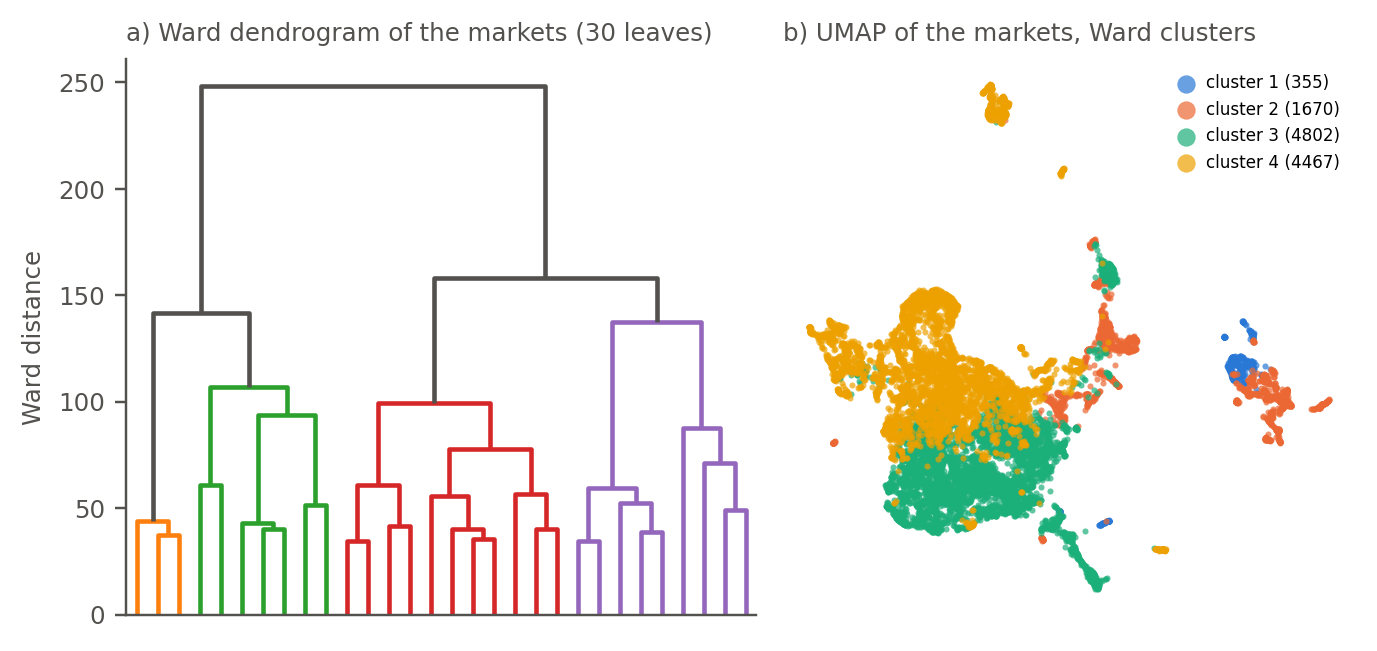
\includegraphics[width=\textwidth]{figures/dm/dm_markets_clusters.png}
\caption{Clustering of the 11{,}294 markets with at least a hundred validation samples at
15 min, on thirteen standardised per-market aggregates (activity, spread, depth, realised
volatility, distance of the mid from one half, share of moving samples, duration, time to
the end, dollars traded, cancellation ratio, contract type).  (a) Ward dendrogram cut at
four clusters; (b) UMAP of the markets coloured by cluster.}
\label{fig:structure:clusters}
\end{figure}

\begin{table}[t]
\centering
\caption{The four Ward clusters of the markets at 15 min: profile (means of the raw
aggregates; the logged quantities are back-transformed), composition by category, and
balanced accuracy of Mean Reversion and of the control inside the cluster.}
\label{tab:structure:clusters}
\small
\begin{fittable}\begin{tabular}{lcccc}
\toprule
& 1 live games & 2 wide-spread & 3 long-dated, mid & 4 long-dated, tight \\
\midrule
markets                           & 355    & 1{,}670 & 4{,}802 & 4{,}467 \\
samples (thousands)               & 748    & 753     & 6{,}333 & 1{,}891 \\
median spread (ticks)             & 3.5    & 33.4    & 9.4     & 0.9 \\
rows in 60 min (geometric mean)   & 320    & 25      & 50      & 16 \\
share of moving samples           & 0.82   & 0.42    & 0.27    & 0.10 \\
hours to the end (median)         & 1.1    & 25      & 1{,}100 & 2{,}300 \\
dollars in 60 min (geometric mean)& 460    & 2       & 0.7     & 1.5 \\
Yes/No contracts                  & 15\%   & 59\%    & 100\%   & 100\% \\
\midrule
sports / esports                  & 288 / 52 & 859 / 153 & 1{,}357 / 21 & 1{,}731 / 39 \\
politics                          & 3      & 120     & 2{,}213 & 1{,}857 \\
economy and tech / crypto         & 1 / 2  & 129 / 128 & 569 / 174 & 339 / 278 \\
weather / culture / other         & 0 / 9 / 0 & 179 / 94 / 8 & 46 / 360 / 62 & 17 / 184 / 22 \\
\midrule
Mean Reversion-$H$                & 0.513  & 0.511   & 0.524   & 0.529 \\
LightGBM G5                       & 0.550  & 0.586   & 0.606   & 0.612 \\
\bottomrule
\end{tabular}\end{fittable}
\end{table}

The markets are the natural unit of this data and \cref{sec:expl:templates} grouped them
by their tags.  \Cref{fig:structure:clusters} groups them instead by how they
trade, on thirteen per-market aggregates of the validation day, with Ward's hierarchical
clustering; $k$-means and HDBSCAN on a five-dimensional UMAP give the same families.  The
silhouette is highest at two clusters ($0.36$) and flat afterwards ($0.13$--$0.16$): the
first split is sharp and the rest is a continuum.  The four-cluster cut of
\cref{tab:structure:clusters} is the readable one.

Cluster 1 is the live games: 355 markets, almost all sports and esports, one hour from
their end, three-tick spreads, three hundred book rows and four hundred dollars an hour,
and a price that moves in 82\% of the 15-minute windows.  Cluster 2 is the wide-spread
markets: 1{,}670 contracts with a median spread of thirty-three ticks, a day from the end,
a mix of sports, weather, esports, crypto and economy, with almost no on-chain trading.
Clusters 3 and 4 are the long-dated markets, political and economic and the pre-game
sports contracts, which differ by their spread: nine ticks against one, and by how often
they move: 27\% against 10\%.  The adjusted mutual information between the clustering and
the category is $0.08$ (Ward), $0.07$ ($k$-means) and $0.10$ (HDBSCAN): the
families cut across the categories, and sports in particular is present in all four.
How a market trades is a different partition from what it is about.

The last two rows are the point of the exercise.  Mean Reversion is within two points of
the same value in every family, but the control is not: $0.550$ in the live games, $0.586$
in the wide-spread markets, $0.606$ and $0.612$ in the long-dated ones.  Predictability at
15 minutes grows as activity falls, and the live games, where almost every window moves and
the direction is the whole problem, are the hardest family even though they are the
richest in data.  This is the per-category table of \cref{sec:horizons:where} seen from
the other side: what makes sports hard is not the sport, it is the live-game regime, and
the pre-game sports contracts in clusters 3 and 4 are as predictable as politics.

\subsubsection{Across the horizons}
\label{sec:structure:horizons}

The study was repeated at every horizon on the samples of the corresponding runs.  What
depends on the features alone does not change: at every horizon four, ten and 22--23
components hold 50, 80 and 95\% of the variance, the effective number of features is
$16.8$--$18.3$, the same fifteen or sixteen correlation blocks appear, a random projection
to twenty dimensions keeps the distances within the same spread and the planar MDS has the
same stress of $0.30$.  The dimensionality is a property of the feature set and of the
validation day, not of the label.  What depends on the label changes in three ways.

\begin{table}[t]
\centering
\caption{Neighbourhood purity lift (same label among the fifteen nearest neighbours over
chance) in the original space / in the UMAP, by horizon.  Only the prediction label
depends on the horizon.}
\label{tab:structure:purityh}
\small
\begin{tabular}{lccccc}
\toprule
Lift of & 1 min & 15 min & 1 h & 6 h & 12 h \\
\midrule
prediction label   & 1.06 / 1.05 & 1.26 / 1.24 & 1.39 / 1.36 & 1.45 / 1.39 & 1.42 / 1.35 \\
market category    & 1.68 / 1.48 & 1.69 / 1.48 & 1.69 / 1.48 & 1.64 / 1.41 & 1.64 / 1.41 \\
price-level bucket & 1.63 / 1.43 & 1.63 / 1.43 & 1.64 / 1.44 & 1.61 / 1.41 & 1.60 / 1.38 \\
activity quartile  & 1.90 / 1.66 & 1.95 / 1.69 & 1.95 / 1.70 & 1.95 / 1.66 & 1.96 / 1.66 \\
market identity    & 216 / 114   & 202 / 104   & 202 / 106   & 198 / 101   & 200 / 102 \\
\bottomrule
\end{tabular}
\end{table}

\paragraph{The label becomes geometric as the horizon grows.}
\Cref{tab:structure:purityh} repeats the purity of \cref{tab:structure:purity} at every
horizon.  The lifts of the category, the price level, the activity and the market identity
are the same at every horizon, as they must be, since the samples are nearly the same.  The
lift of the label is $1.06$ at 1 min, $1.26$ at 15 min, $1.39$ at 1 h and $1.42$--$1.45$
at 6 and 12 h.  At one minute the neighbours of a sample carry almost no information on
its label: whether the price moves in the next minute is a matter of the next book event,
not of where the sample sits in the feature space.  At twelve hours the neighbourhood is
informative, and the information is about the direction, because the \textsc{const}
class has become a third of the samples.

\begin{table}[t]
\centering
\caption{Separability by horizon: balanced accuracy on all and deduplicated samples of the
same learners as \cref{tab:structure:sep15}.  kNN with the best $k$ on 300{,}000
samples; $\Delta$ is the difference from the control on the same samples, hour-block
bootstrap 95\% interval.}
\label{tab:structure:seph}
\footnotesize
\begin{fittable}\begin{tabular}{lcccccccccc}
\toprule
& \multicolumn{2}{c}{1 min} & \multicolumn{2}{c}{15 min} & \multicolumn{2}{c}{1 h} & \multicolumn{2}{c}{6 h} & \multicolumn{2}{c}{12 h} \\
\cmidrule(lr){2-3}\cmidrule(lr){4-5}\cmidrule(lr){6-7}\cmidrule(lr){8-9}\cmidrule(lr){10-11}
Model & all & dedup & all & dedup & all & dedup & all & dedup & all & dedup \\
\midrule
Mean Reversion-$H$     & 0.536 & 0.501 & 0.537 & 0.525 & 0.531 & 0.518 & 0.507 & 0.500 & 0.507 & 0.500 \\
LDA                    & 0.462 & 0.362 & 0.561 & 0.495 & 0.563 & 0.546 & 0.541 & 0.517 & 0.539 & 0.516 \\
Logistic regression    & 0.504 & 0.376 & 0.568 & 0.505 & 0.562 & 0.525 & 0.544 & 0.518 & 0.543 & 0.519 \\
Decision tree, depth 3 & 0.558 & 0.474 & 0.548 & 0.549 & 0.534 & 0.503 & 0.513 & 0.492 & 0.499 & 0.497 \\
Decision tree, depth 6 & 0.575 & 0.479 & 0.571 & 0.562 & 0.554 & 0.535 & 0.531 & 0.512 & 0.531 & 0.523 \\
kNN, best $k$          & 0.508 & 0.400 & 0.574 & 0.553 & 0.566 & 0.549 & 0.543 & 0.528 & 0.546 & 0.533 \\
\quad best $k$ & \multicolumn{2}{c}{20} & \multicolumn{2}{c}{200} & \multicolumn{2}{c}{200} & \multicolumn{2}{c}{1000} & \multicolumn{2}{c}{1000} \\
\quad $\Delta$ vs control & \multicolumn{2}{c}{$-10.2$ [$-11.2$, $-9.5$]} & \multicolumn{2}{c}{$-4.0$ [$-4.3$, $-3.8$]} & \multicolumn{2}{c}{$-3.6$ [$-4.0$, $-3.2$]} & \multicolumn{2}{c}{$-3.0$ [$-3.3$, $-2.6$]} & \multicolumn{2}{c}{$-2.5$ [$-2.8$, $-2.2$]} \\
LightGBM G5 (control)  & 0.609 & 0.474 & 0.616 & 0.600 & 0.602 & 0.583 & 0.572 & 0.567 & 0.572 & 0.568 \\
\bottomrule
\end{tabular}\end{fittable}
\end{table}

\begin{figure}[t]
\centering
\begin{tikzpicture}
\begin{axis}[thesis, width=0.62\textwidth, height=5.4cm, xmode=log, log basis x=10, xlabel={$k$ (neighbours)}, ylabel={balanced accuracy, all samples}, xmin=3, xmax=1600, ymin=0.44, ymax=0.70, legend pos=outer north east, legend columns=1, legend cell align=left]
\addplot[vizA, thick, mark=*, mark size=1.6pt] coordinates {(5,0.4913) (20,0.5084) (50,0.5015) (200,0.4919) (1000,0.4692)};
\addlegendentry{kNN 1 min}
\addplot[vizB, thick, mark=square*, mark size=1.6pt] coordinates {(5,0.5324) (20,0.5597) (50,0.5702) (200,0.5743) (1000,0.5719)};
\addlegendentry{kNN 15 min}
\addplot[vizC, thick, mark=triangle*, mark size=1.6pt] coordinates {(5,0.5200) (20,0.5498) (50,0.5593) (200,0.5664) (1000,0.5646)};
\addlegendentry{kNN 1 h}
\addplot[vizD, thick, mark=diamond*, mark size=1.6pt] coordinates {(5,0.4972) (20,0.5197) (50,0.5323) (200,0.5402) (1000,0.5431)};
\addlegendentry{kNN 6 h}
\addplot[vizInk, thick, mark=pentagon*, mark size=1.6pt] coordinates {(5,0.5023) (20,0.5272) (50,0.5370) (200,0.5460) (1000,0.5460)};
\addlegendentry{kNN 12 h}
\end{axis}
\end{tikzpicture}

\caption{Balanced accuracy of the balanced-vote kNN against $k$ at every horizon, on
300{,}000 validation samples.  The optimum moves from $k = 20$ at 1 min to $k = 1000$ at
6 and 12 h.}
\label{fig:structure:knn}
\end{figure}

\paragraph{The short horizons are a threshold problem, the long ones a linear one.}
\Cref{tab:structure:seph} and \cref{fig:structure:knn} order the simple learners
differently at each end of the range.  At 1 min the linear models are \emph{below} Mean
Reversion ($0.462$ and $0.504$ against $0.536$) and the nearest-neighbour classifier
reaches $0.508$ at its best $k = 20$, ten points under the control; the only simple
learners that work are the trees, and a depth-three tree with its first split at
``no move in the last 105 seconds'' is at $0.558$, one point from the depth-six tree and
five from the control.  Every learner, the control included, falls to $0.47$--$0.48$ on
the deduplicated samples at this horizon.  At 15 min the trees are still ahead of the
linear and local learners.  At 1 h the order reverses: linear discriminant analysis, at
$0.563$ on all samples and $0.546$ deduplicated, is the best simple learner, above the
depth-six tree ($0.554$ / $0.535$) and level with kNN, and it matches to the third decimal
the LOB-only stateful model with the time-first encoder of mid-October, evaluated on the
same samples ($0.564$ / $0.541$,
\cref{sec:stateful:encoders}).  At 6 and 12 h the linear models and kNN are together at
$0.54$, the trees below them, and the margin of the control shrinks to $2.5$--$3$ points.
The gap between the control and the best simple learner goes from ten points at 1 min to
two and a half at 12 h: the boosted trees earn their advantage where the problem is made
of thresholds on the activity clock, and the threshold itself scales with the horizon:
the first split of the depth-three tree is at 105 seconds since the last move at 1 min,
17 minutes at 15 min, 3.1 hours at 6 h and 5.5 hours at 12 h.

\begin{table}[t]
\centering
\caption{Mutual information between a feature and the label, in nats, by horizon, for the
fifteen features that are among the six most informative at some horizon (bold where they
are), and the sum over each group.  300{,}000 validation samples, nearest-neighbour
estimator.  Label entropy 0.42, 0.83, 1.00, 1.10, 1.09 nats.}
\label{tab:structure:mih}
\small
\begin{tabular}{lccccc}
\toprule
Feature (group) & 1 min & 15 min & 1 h & 6 h & 12 h \\
\midrule
\path{moves_60m} (G3) & \textbf{0.149} & \textbf{0.221} & \textbf{0.212} & 0.135 & 0.104 \\
\path{rv_60m} (G3) & \textbf{0.142} & \textbf{0.229} & \textbf{0.225} & 0.154 & 0.122 \\
\path{since_move} (G3) & \textbf{0.123} & \textbf{0.209} & \textbf{0.211} & 0.167 & 0.153 \\
\path{range_pos_60m} (G3) & \textbf{0.132} & \textbf{0.182} & 0.171 & 0.110 & 0.090 \\
\path{mid_minus_mean60} (G3) & 0.104 & \textbf{0.187} & \textbf{0.190} & 0.127 & 0.099 \\
\path{usd_15m} (G4) & \textbf{0.112} & 0.114 & 0.099 & 0.062 & 0.055 \\
\path{ntr_15m} (G4) & \textbf{0.105} & 0.088 & 0.070 & 0.032 & 0.028 \\
\path{ret_15m} (G1) & 0.097 & 0.162 & 0.143 & 0.080 & 0.060 \\
\path{ret_1h} (G1) & 0.087 & 0.158 & 0.165 & 0.112 & 0.089 \\
\path{micro_minus_mid_ticks} (G2) & 0.044 & \textbf{0.166} & \textbf{0.270} & \textbf{0.410} & \textbf{0.457} \\
\path{imb1} (G2) & 0.041 & 0.143 & \textbf{0.233} & \textbf{0.362} & \textbf{0.408} \\
\path{log_bid_sz0} (G2) & 0.039 & 0.116 & 0.184 & \textbf{0.290} & \textbf{0.334} \\
\path{log_ask_sz0} (G2) & 0.035 & 0.100 & 0.160 & \textbf{0.261} & \textbf{0.303} \\
\path{log_bid_sz10} (G2) & 0.024 & 0.085 & 0.139 & \textbf{0.217} & \textbf{0.242} \\
\path{log_duration_h} (G5) & 0.095 & 0.148 & 0.178 & \textbf{0.223} & \textbf{0.262} \\
\midrule
sum over G1 (price) & 0.63 & 1.16 & 1.31 & 1.16 & 1.10 \\
sum over G2 (book) & 0.38 & 1.10 & 1.68 & 2.51 & 2.81 \\
sum over G3 (flow and clock) & 1.15 & 1.45 & 1.38 & 0.87 & 0.73 \\
sum over G4 (trades) & 0.60 & 0.75 & 0.76 & 0.51 & 0.46 \\
sum over G5 (static) & 0.28 & 0.37 & 0.42 & 0.45 & 0.49 \\
\bottomrule
\end{tabular}
\end{table}

\paragraph{The information moves from the clock to the book.}
\Cref{tab:structure:mih} is the clearest statement of the horizon dependence in the
thesis.  At 1 and 15 min the most informative features are the activity clock: the
sixty-minute number of moves, the realised volatility, the time since the last move, the
position in the range; the flow-and-clock group sums to $1.15$ and $1.45$ nats and the
book-shape group to $0.38$ and $1.10$.  From 1 h the order turns: the microprice offset
and the first-level imbalance lead, followed by the sizes at the first level, and the
book-shape group sums to $1.68$ nats at 1 h, $2.51$ at 6 h and $2.81$ at 12 h, while the
clock falls to $0.73$.  The price group is stable at $1.1$--$1.3$ nats and the duration of
the market is in the top six from 6 h onward.  The reading is the one of
\cref{sec:expl:direction}: at short horizons the question is whether the price will move
and the clock answers it; at long horizons almost every price moves, the question is the
direction, and the shape of the book, which is strongly conditioned by the price level
(\cref{sec:expl:level}), is what carries it.  The same features, the same day: what the
label asks of them changes with $H$, and so does which model family can read them.

\paragraph{The families of markets, by horizon.}  The clustering of
\cref{sec:structure:markets} was repeated on the samples of each horizon; since the share
of moving samples is one of the aggregates, the partition is re-derived each time and the
clusters are not identical across horizons.  The live-game family is recovered at 1 min
(304 markets), 15 min (355) and 1 h (356), always sports and esports an hour from the end;
at 6 and 12 h it merges with the wide-spread sports contracts into a family of 648 and 566
markets.  The control inside the live games is $0.573$ at 1 min, $0.550$ at 15 min,
$0.548$ at 1 h, and $0.476$ and $0.488$ at 6 and 12 h, where Mean Reversion in the same
family is at $0.42$ and $0.38$: in a game that is ending, the price trends, and the
reversal rule is wrong more often than right.  At the other end, a family of deep and
tight long-dated markets (368 markets at 1 min, 527 at 12 h; spreads under one tick,
first-level depth of thousands of shares) is the \emph{worst} family for the control at 1
min, $0.412$ against $0.527$ for Mean Reversion, because its price moves in 2\% of the
minutes and the control cannot pick them, and the \emph{best} family at 12 h, $0.614$:
the deep markets are the ones whose direction over a day is readable in the book.  The
adjusted mutual information between the families and the category stays between
$0.04$ and $0.10$ at every horizon.

